% XeLaTeX can use any Mac OS X font. See the setromanfont command below.
% Input to XeLaTeX is full Unicode, so Unicode characters can be typed directly into the source.

% The next lines tell TeXShop to typeset with xelatex, and to open and save the source with Unicode encoding.

%!TEX TS-program = xelatex
%!TEX encoding = UTF-8 Unicode

\documentclass[12pt]{article}
\usepackage{geometry}                % See geometry.pdf to learn the layout options. There are lots.
\geometry{letterpaper}                   % ... or a4paper or a5paper or ... 
%\geometry{landscape}                % Activate for for rotated page geometry
%\usepackage[parfill]{parskip}    % Activate to begin paragraphs with an empty line rather than an indent
\usepackage{graphicx}
\usepackage{indentfirst}
\usepackage{listings}
\usepackage{amssymb}
\usepackage{enumerate}
\usepackage{amsmath}
\usepackage{float}

% Will Robertson's fontspec.sty can be used to simplify font choices.
% To experiment, open /Applications/Font Book to examine the fonts provided on Mac OS X,
% and change "Hoefler Text" to any of these choices.

\usepackage{fontspec,xltxtra,xunicode}
\defaultfontfeatures{Mapping=tex-text}
\setromanfont[Mapping=tex-text]{Times New Roman}
\setsansfont[Scale=MatchLowercase,Mapping=tex-text]{Hiragino Sans GB}
\setmonofont[Scale=MatchLowercase]{Andale Mono}
\lstset{language=Python, basicstyle=\tiny}

\title{Applied Mathematics for Computer Science: \\Experiment Report}
\author{Yuwen Xiong\\3130000829}
%\date{}                                           % Activate to display a given date or no date

\begin{document}
\maketitle

\section{Homework 1} 

We generate a $\sin$ curve in $[0, 1]$ with $N(0, 0.1)$ gaussian noise by following code:
\begin{lstlisting}[frame=single]
    sample_x = np.linspace(0, 1, n)
    sample_y = np.sin(sample_x * 2 * np.pi) + np.random.normal(0, 0.1, n)
\end{lstlisting}

We just calculate the close form $w = (X^TX + \lambda I)^{-1}X^Ty$ to get the corresponding $w$, and plot it.

\begin{figure}[hbtp]
  \centering
  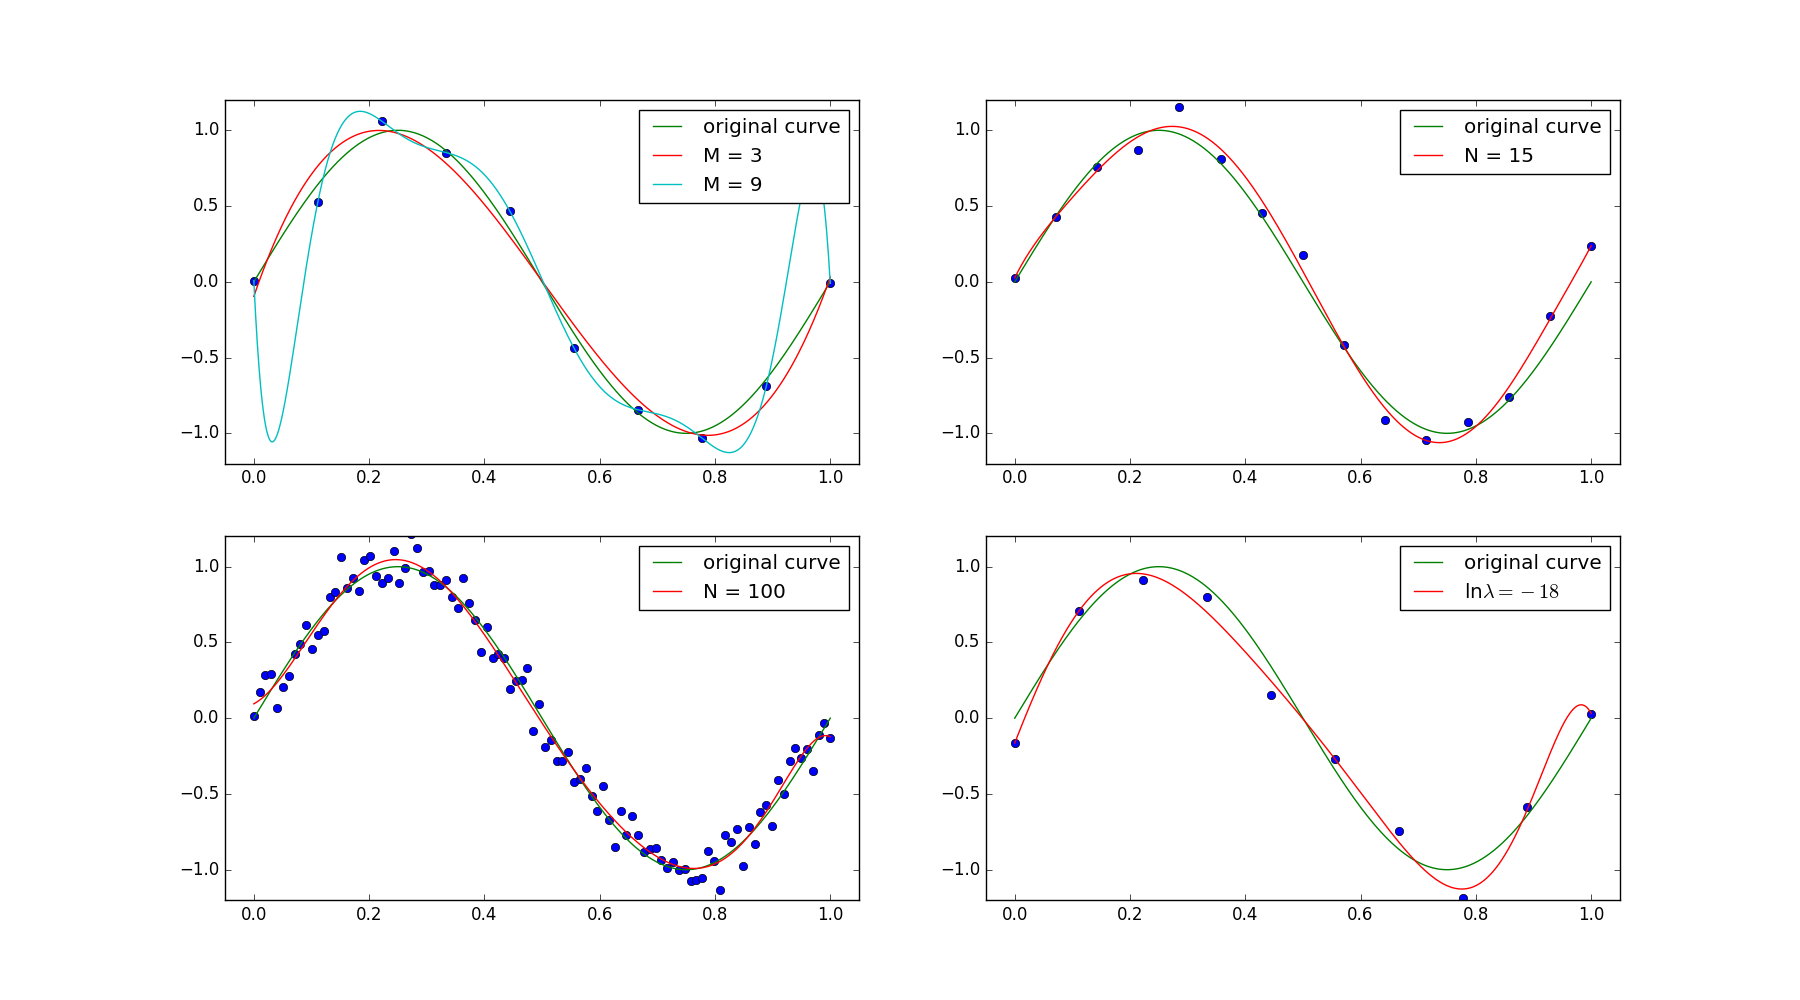
\includegraphics[width=12.5cm]{hw1_result.png}
  \caption{The result of homework 1}
\end{figure}


\section{Homework 2}

We use {\em optdigits.tes} as input, reduce its dimension from 64 to 2 by SVD decomposition and visualize them in 2D plot. 

The key code as follows:

\begin{lstlisting}[frame=single]
    m = feas.mean(axis = 0)
    feas = (feas - m)
    U, S, VT = np.linalg.svd(feas, full_matrices = False)
    res = np.dot(U[:, 0:2], np.diag(S[0:2]))
\end{lstlisting}

\begin{figure}[hbt]
  \centering
  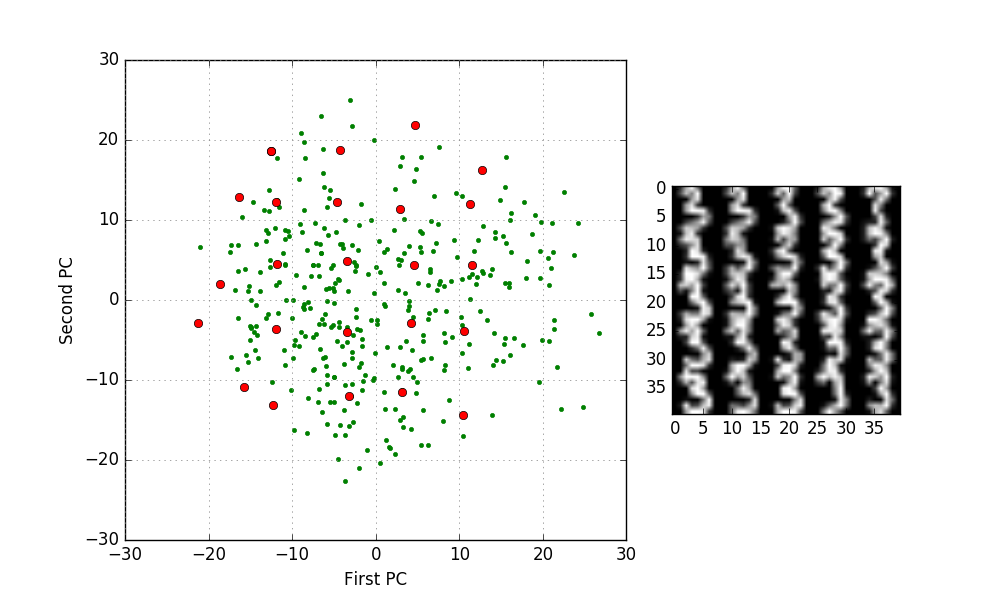
\includegraphics[width=\textwidth]{hw2_result.png}
  \caption{The result of homework 2}
\end{figure}


\section{Homework 3}

We use {\em numpy.random.multivariate\_normal} as follows to generate three 2-D multivariable gaussian clusters, and implement a mog class with EM algorithm.

\begin{lstlisting}[frame=single]
    mean1 = [3, 0]
    mean2 = [-1, -3]
    mean3 = [4, 5]
    sigma1 = np.diag((1, 4))
    sigma2 = np.diag((4, 3))
    sigma3 = np.array([[2, 1], [1, 2]])

    norm1 = np.random.multivariate_normal(mean1, sigma1, 300)
    norm2 = np.random.multivariate_normal(mean2, sigma2, 300)
    norm3 = np.random.multivariate_normal(mean3, sigma3, 300)
\end{lstlisting}

We also implement {\em regularization term support} and we think our code could also handle {\em higher dimensional} data(though we haven't tested it).


\begin{figure}[htbp]
  \centering
  \begin{minipage}[t]{0.48\linewidth}
      \centering
	  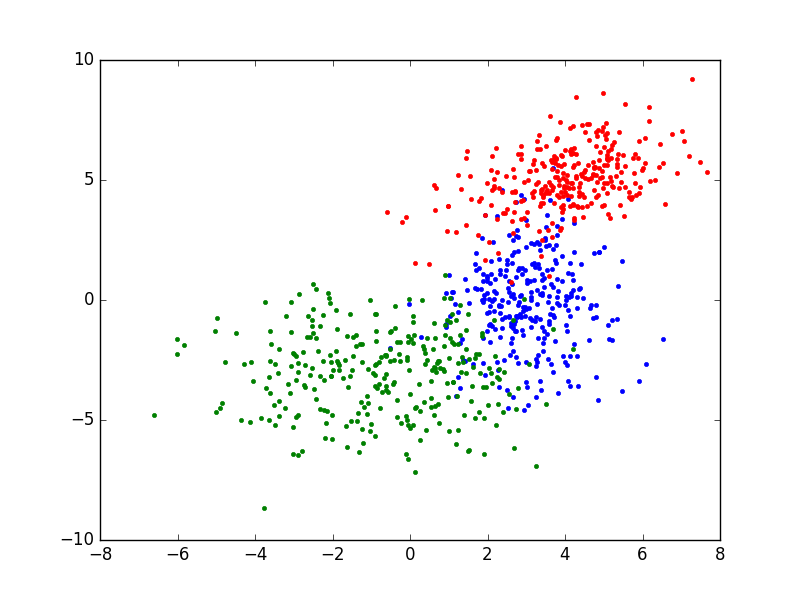
\includegraphics[width=8cm]{hw3_original.png}
	  \caption{The original data}  	
  \end{minipage}
  \hfill
  \begin{minipage}[t]{0.48\linewidth}
      \centering
      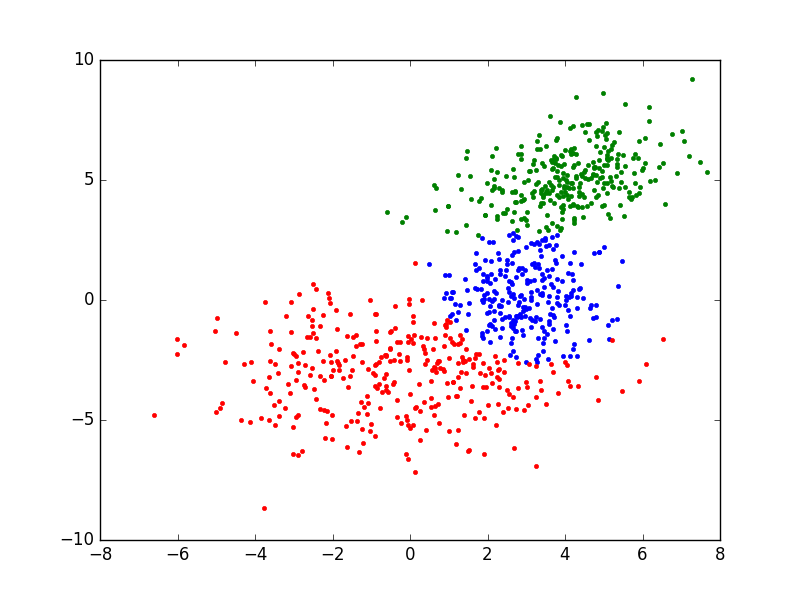
\includegraphics[width=8cm]{hw3_result_reg=0.png}
	  \caption{The result generated with reg$=0$}  	
  \end{minipage}
  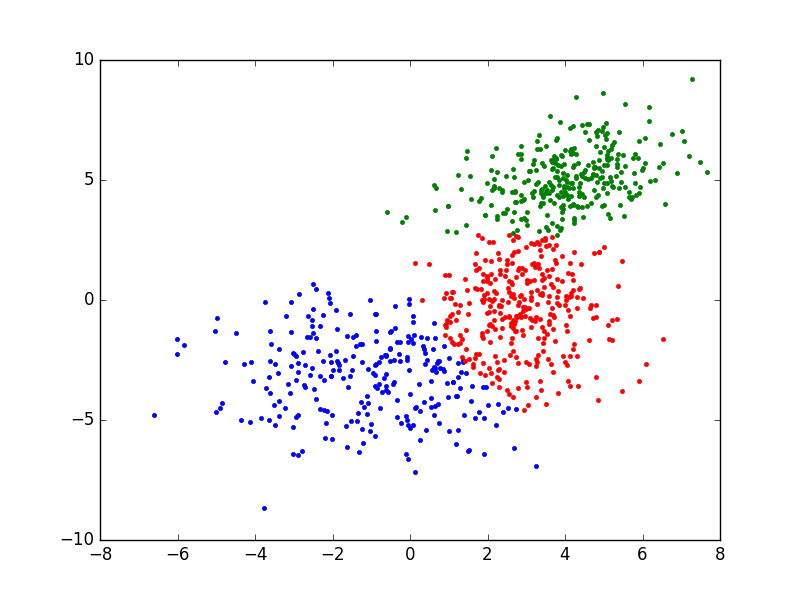
\includegraphics[width=8cm]{hw3_result_reg=0.2.png}
  \caption{The result generated with reg$=0.2$}
\end{figure}
%\begin{figure}[hbtp]
%\end{figure}
%\begin{figure}[hbtp]
%\end{figure}

As we can see, reg=0.2 produce a better result than reg = 0.

\section{Homework 4}

We implement the Levenberg-Marquardt method to solve the extremum problem.

We use $\sin(x) + \cos(y)$ and $\frac{1}{4}x^4 - \frac{1}{3}x^3 + \frac{1}{2}x^2 - x + 1$ as our target function, and visualize the first one.

\begin{figure}[hbtp]
  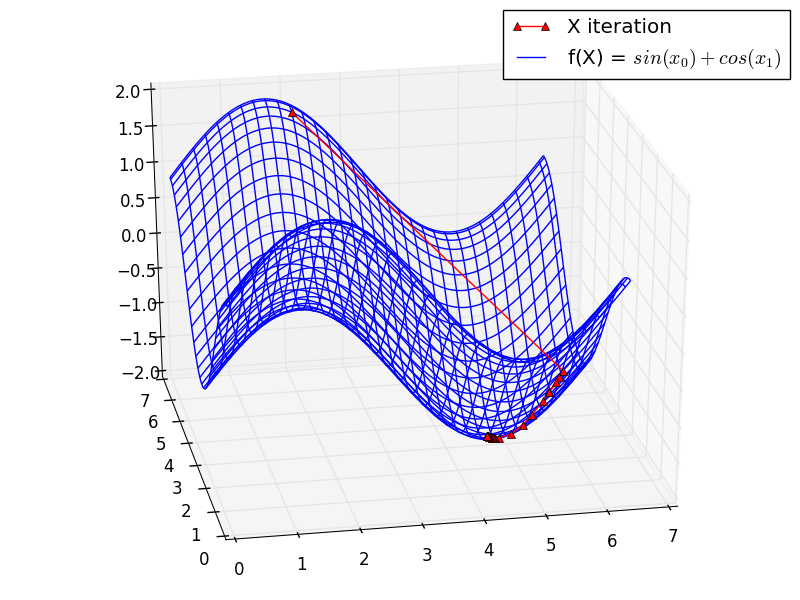
\includegraphics[width=\textwidth]{hw4_result.png}
  \caption{The result of homework 4}
\end{figure}

We observed a strange phenomenon: when we fix r = 1,  it will converge much faster, we haven't figure it out till now.


\section{Homework 5}

We implement the primal SVM with active set method, since active set method needs a valid initial value, we use cvxopt to solve a linear programming to get a initial value.

\begin{figure}[hbt]
  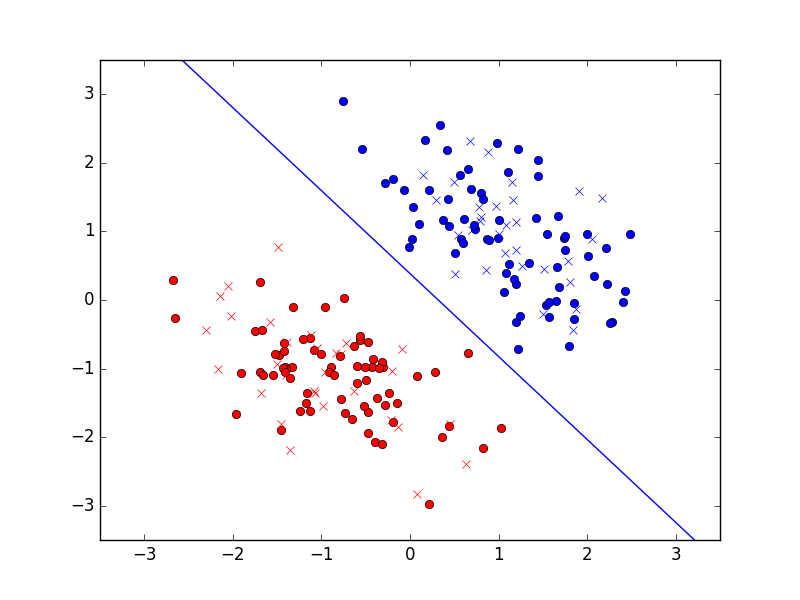
\includegraphics[width=\textwidth]{hw5_result.png}
  \caption{The result of homework 5}
\end{figure}



\end{document}  